\documentclass[11pt]{article}
\usepackage[letterpaper,margin=1in]{geometry}
\usepackage[T1]{fontenc}
\usepackage{lmodern,microtype,amsmath,amssymb,graphicx,booktabs,array}
\usepackage[colorlinks=true,urlcolor=blue,citecolor=blue,linkcolor=blue]{hyperref}
\usepackage{caption}
\usepackage{fancyhdr,placeins}
\hypersetup{pdftitle={From Dated Ties to Defensible Routes},pdfauthor={Shivam Gupta}}
\captionsetup{font=small,labelfont=bf}
\pagestyle{fancy}\fancyhf{}\lhead{Gupta | From Dated Ties to Defensible Routes}\rhead{\thepage}
\renewcommand{\headrulewidth}{0.3pt}
\setlength{\headheight}{14pt}
\setlength{\parskip}{4pt}
\setlength{\parindent}{0pt}
\setlength{\emergencystretch}{2em}
\makeatletter
\setlength{\@fptop}{0pt}
\setlength{\@fpsep}{18pt}
\setlength{\@fpbot}{0pt plus 1fil}
\makeatother
\title{\textbf{From Dated Ties to Defensible Routes}\\[4pt]\large A Handoff-Feasibility Audit of Revolutionary Correspondence, 1771--1783}
\author{Shivam Gupta\\\small Independent Researcher, India\\\small\href{mailto:shivam1720406@gmail.com}{shivam1720406@gmail.com}}
\date{14 October 2026}
\begin{document}
\maketitle
\begin{abstract}
Historical correspondence graphs make communication pathways visible, but a document date does not establish receipt or transmission of shared information. We present DispatchGap, an executable audit that separates aggregate connectivity, date-ordered routes, and routes satisfying a specified minimum inter-document handoff gap. The audit retains document identifiers, permits explicit corpus exclusions, and returns inspectable route witnesses and critical-gap thresholds. Applied to a pinned release of Revolutionary Networks, 40,659 usable documents connect 5,009 identifiers. Across thirteen annual windows, directed aggregate graphs contain 3,578,961 reachable ordered pairs. Date ordering retains 59.78\%; seven-day and thirty-day minimum gaps retain 55.45\% and 43.38\%, respectively. Thirty-day gaps remove 27.43\% of the pairs admitted by date ordering alone. Removing records with repeated Founders Online links has little effect; other document exclusions produce appreciably different opportunity graphs. An independent finite-state oracle verifies 55,575 origin-stream-gap cases. The contribution is a source-linked feasibility benchmark and reusable interpretive workflow built on established temporal-network methods. Its conclusions concern admissible routes through recorded documents; assertions about actual circulation still require evidence of receipt, content, and archival coverage.
\end{abstract}
\noindent\textbf{Keywords:} historical network analysis; correspondence; early America; temporal reachability; source criticism; reproducible software

\section{The chronological promise of a network}
A synthetic history can connect places, people, and institutions across documentary collections that no participant experienced as a single archive. Correspondence networks offer a powerful instrument for that work. A line between two names makes a relationship legible; a chain of lines suggests a route along which news, instructions, or arguments might have travelled. The second interpretation requires more evidence than the first. A recipient must have had access to an earlier communication before producing a later one, and an account of influence must connect their contents. The date attached to an edited document establishes neither condition by itself.

This distinction becomes consequential when a visualization supplies a compact explanation of historical integration. An aggregate graph can connect people through documents written in the wrong order. A date-ordered graph removes that contradiction while allowing a recipient to act immediately. Neither the historian nor the software needs to believe that instantaneous transmission occurred for the assumption to shape the result. It can enter through the apparently routine choice to represent a dated letter as a contact event.

The question addressed here is operational: how much of a founding-era opportunity graph survives when its recorded contacts must leave time between successive documents? A second question concerns interpretability: can the resulting calculation return the specific records and temporal restriction responsible for a proposed route? DispatchGap treats both questions as source-critical tasks. It supplies an exact audit of a declared representation, with outputs that lead back to documentary identifiers rather than a freestanding numerical claim about historical connectedness.

The case is Revolutionary Networks, a public metadata compilation released by the University of Virginia Press's Rotunda imprint in 2026 \cite{rotunda}. Its scope, 1771--1783, spans the transition from colonial controversy to revolutionary war and independence. This study evaluates the compilation as a research object. It does not reconstruct the complete correspondence of the period or identify the diffusion of a particular political idea. The object is sufficiently substantial to expose the consequences of representation while keeping the documentary limits visible.

\section{Position within existing scholarship}
Temporal-network research establishes that connectivity depends on the sequence of contacts \cite{holme}. Minimum waiting constraints, traversal times, and label-setting methods also have substantial algorithmic histories \cite{bazgan}. The computation here specializes those ideas to dated documentary records. There is no claim of priority for temporal reachability, minimum handoff constraints, or binary search over a monotone feasibility condition.

Humanistic network scholarship supplies the interpretive problem. Ahnert and colleagues describe the movement between richer documentary representations and more tractable graphs, emphasizing that even a temporal network leaves out a letter's textual and material circumstances \cite{ahnert}. Their account makes source criticism integral to the choice of representation. DispatchGap provides one concrete way to examine a consequence of that choice, with numerical outputs linked to the documents that generate them.

Recent epistolary infrastructure supports the preservation and analysis of rich metadata. Leskinen and colleagues connect historical knowledge graphs with temporal communication analysis across several substantial collections \cite{leskinen}. Ure\~na-Carrion and colleagues compare historical and contemporary communication using aggregate networks, inter-event times, and social signatures; they explicitly recognize the logistical constraints on epistolary timing \cite{urena}. The present audit asks a different empirical question about admissible multi-document routes. Alassi and Rosenthaler develop RDF-based editions that distinguish multiple layers of correspondence data \cite{alassi}. An's CIDOC CRM study further demonstrates the importance of representing temporal uncertainty \cite{an}.

Archival coverage poses an additional limitation that temporal computation cannot repair. Kane's analysis of women's correspondence in Founders Online shows how collection and editorial histories shape the networks available for study \cite{kane}. Consequently, a missing route in a compilation can direct further inquiry, but cannot establish that people lacked contact. This study places the temporal restriction and the coverage restriction alongside one another: the first can be computed exactly for the released records, whereas the second requires historical investigation.

The specific contribution is a complete, reproducible route-feasibility audit of the pinned Revolutionary Networks release, together with source-level witnesses, explicit terminal-leg semantics, and controlled document exclusions. The literature search found strong precedents for the components, rather than evidence supporting a claim that the general problem was previously unrecognized. The contribution's significance rests on the empirical reconstruction and its reusable workflow.

\section{Data and a declared route model}
The frozen CSV contains 40,690 rows with unique document identifiers. It supplies author and recipient identifier lists, an associated date, publication labels, source links, and location metadata. Analysis uses repository commit \texttt{dacbbff} and records the full SHA-256 digest in the accompanying manifest. All dates parse as calendar days within the stated period. Twenty-two records lack author identifiers and nine more lack recipient identifiers; these 31 records are excluded from route construction.

Semicolon-separated identifier lists are interpreted as sets within each document. Six repeated identifier tokens are removed by that operation. The resulting 40,659 documents involve 5,009 unique identifiers; 2,028 documents have multiple distinct authors or recipients. Cartesian author-to-recipient expansion produces 45,070 contact instances, including 153 self-contacts. Removing self-contacts leaves 44,917 directed instances. Each retains its originating document identifier. Expansion declares possible dyadic contacts from the recorded lists; it does not establish separate physical deliveries to every addressee.

For each calendar year, the vertex set contains identifiers appearing in that year's usable records. Annual windows keep the horizon consistent and avoid attributing cross-year routes to a single year's graph. A route is a sequence of contacts $e_1,\ldots,e_k$, with each recipient identical to the next author. If $t_i$ is the calendar-day index of contact $e_i$, a route satisfies minimum gap $g$ when
\begin{equation}
 t_{i+1}-t_i\geq g\quad\text{for every }i<k.
\end{equation}
The audit evaluates integer gaps of 0, 1, 3, 7, 14, 30, and 60 days. These are sensitivity settings, not reconstructed postal transit times. The zero-gap case permits same-day chains; its within-day closure is independent of CSV row order. Positive gaps prohibit reuse of a document as successive steps on the same date.

The terminal leg receives special treatment. The question is whether the recorded sequence can end with a document dated inside the window. The final recipient need not become available for another step before December 31. Thus a direct contact remains admissible at every gap, and a final-year document is not discarded because an assumed transit duration extends past the window. Every origin is hypothetically available at the window's start; the calculation carries distinct origin labels, rather than modeling a jointly observed spreading episode.

Let $R_y^{\mathrm{agg}}$ be the set of non-self ordered pairs joined by the directed aggregate graph in year $y$, and $R_y(g)$ those admitting a gap-constrained route. The pooled retention statistic is
\begin{equation}
 Q(g)=\frac{\sum_y |R_y(g)|}{\sum_y |R_y^{\mathrm{agg}}|}.
\end{equation}
A pair appearing in two years contributes twice. This is a source-year statistic, weighted by the number of aggregate-reachable pairs, rather than a fraction of unique people or a mean of annual percentages. Unlimited waiting is permitted. Receipt, reading, forwarding, and content continuity remain unobserved.

\section{Executable computation and verification}
DispatchGap computes all origins simultaneously using integer bitsets. Each vertex initially contains its own origin label. At a document date, an author's available labels can reach the recipient as terminal labels. They become available for further transmission after $g$ days. A priority queue processes these delayed availability events before contacts on the same date. For zero gap, repeated relaxation computes the day's directed closure. This distinction prevents a file's sorting convention from determining same-day reachability.

Correctness follows from a chronological invariant: immediately before a dated contact is processed, a vertex's availability set contains exactly the origins with an admissible prefix ready by that date. A processed contact extends every such prefix; delayed availability forbids premature onward steps. Conversely, the final contact of any admissible route extends a prefix already available when that contact is processed. Same-day closure supplies the corresponding invariant when the gap is zero. The released implementation and an independent state-space oracle make this argument testable.

Feasibility is monotone: increasing $g$ can only remove routes. For an indirectly connected pair, define its critical gap by
\begin{equation}
 \Gamma_y(s,z)=\max_{p:s\leadsto z}\min_{i<|p|}(t_{i+1}-t_i).
\end{equation}
An unreachable pair has no threshold; a pair with a direct contact has unbounded threshold under the terminal-leg convention. For other pairs, integer binary search finds the largest feasible gap. A document sequence demonstrates feasibility at that threshold; an exact reachability computation establishes failure at the next integer. The threshold refers to all admissible routes, rather than merely the weakest transition on one arbitrarily selected route.

Verification enumerates every ordered stream of up to three contacts on three vertices and three dates, testing three gaps and every origin. All 55,575 origin-stream-gap comparisons agree with a separate search over vertex-and-availability states. Returned witnesses are checked for matching endpoints and valid successive date gaps. Additional tests cover last-day terminal legs, critical thresholds, monotonicity, and invariance under shuffled input order. The oracle also agrees in nine checks on complete 1771, 1776, and 1781 graphs, using each year's most frequently documented identifier at gaps 0, 7, and 30. Full-corpus checks verify set inclusion in aggregate reachability and monotonicity across all tested gaps.

\section{Results: connectedness changes with the question}
Across thirteen annual graphs, aggregate connectivity admits 3,578,961 ordered source-year pairs. Date ordering retains 2,139,654, or 59.78\%. Consequently, 40.22\% of aggregate-connected pairs lack even a nondecreasing document-date route within their year. Seven-day gaps admit 1,984,485 pairs; thirty-day gaps admit 1,552,670. Relative to date ordering alone, those settings remove 7.25\% and 27.43\%, respectively. Table~\ref{tab:pooled} and Figure~\ref{fig:reach} report the full curve.

\begin{table}[htbp]\centering\small
\caption{Pooled annual reachability. The fixed denominator is 3,578,961 directed aggregate-reachable source-year pairs.}\label{tab:pooled}
\begin{tabular}{rrr}\toprule Minimum gap (days)&Admissible pairs&Aggregate pairs retained\\\midrule
0&2,139,654&59.78\%\\1&2,116,575&59.14\%\\3&2,072,392&57.90\%\\7&1,984,485&55.45\%\\14&1,842,923&51.49\%\\30&1,552,670&43.38\%\\60&1,110,050&31.02\%\\\bottomrule\end{tabular}
\end{table}
\begin{figure}[htbp]\centering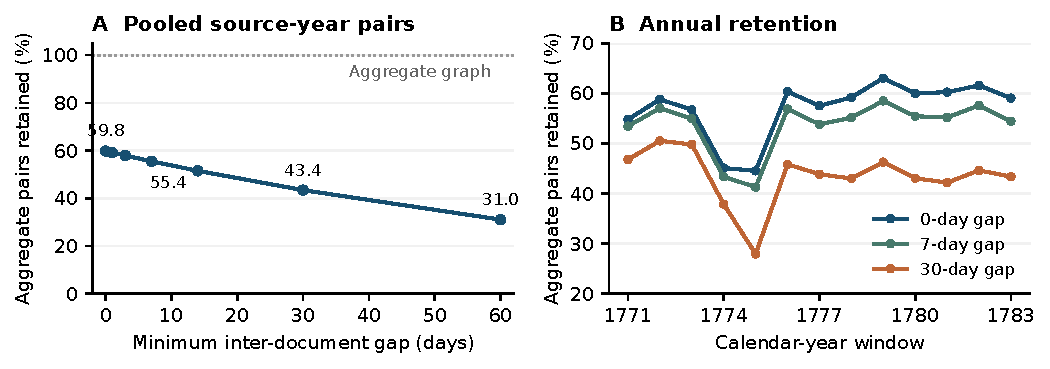
\includegraphics[width=\linewidth]{figures/reachability.pdf}
\caption{Pooled and annual retention under minimum inter-document gaps. Annual denominators differ; the pooled curve counts source-year pairs. All results concern the recorded opportunity graph.}\label{fig:reach}\end{figure}

Annual zero-gap retention ranges from 44.51\% in 1775 to 63.02\% in 1779. This variation cannot be interpreted directly as changing political cohesion. The compilation's annual sizes, editorial coverage, and patterns of correspondence differ substantially. The calculation identifies how the temporal representation changes each opportunity graph, leaving the historical explanation of those differences open to source investigation.

Controlled exclusions retain each full annual vertex set and its aggregate denominator. Restricting to singleton-author, singleton-recipient documents yields pooled zero-gap retention of 50.23\% and thirty-day retention of 36.60\%. Excluding documents involving identifiers prefixed \texttt{RN-ORG-} yields 53.66\% and 39.10\%; excluding rows labeled \texttt{EA} yields 46.17\% and 33.18\%. These comparisons measure the consequences of deleting defined documentary classes. They do not classify those classes as unreliable, or isolate an independent causal contribution of institutions or editorial status.

Link-based deduplication has a substantially smaller effect: zero-gap retention changes from 59.784\% to 59.772\%, and thirty-day retention from 43.383\% to 43.373\%. Matching a source URL is a deliberately narrow rule; it does not identify every document that represents the same historical communication. Nevertheless, ordinary repeated-link removal does not explain the main reachability differences.

An exploratory timing control permutes usable documents' dates within their calendar years for twenty deterministic seeds. It preserves documents, endpoints, annual membership, and the document-date multiset, while breaking their observed association. Group documents retain a common assigned date across projected contacts. Pooled zero-gap reachability ranges from 2,331,119 to 2,392,804 across these controls, above the observed 2,139,654. At thirty days the range is 1,735,069--1,793,901, again above the observed 1,552,670. The result demonstrates sensitivity to the observed ordering. These permutations are diagnostic constructions, not reconstructed alternative histories or a sampling distribution for unobserved letters.

\begin{figure}[htbp]\centering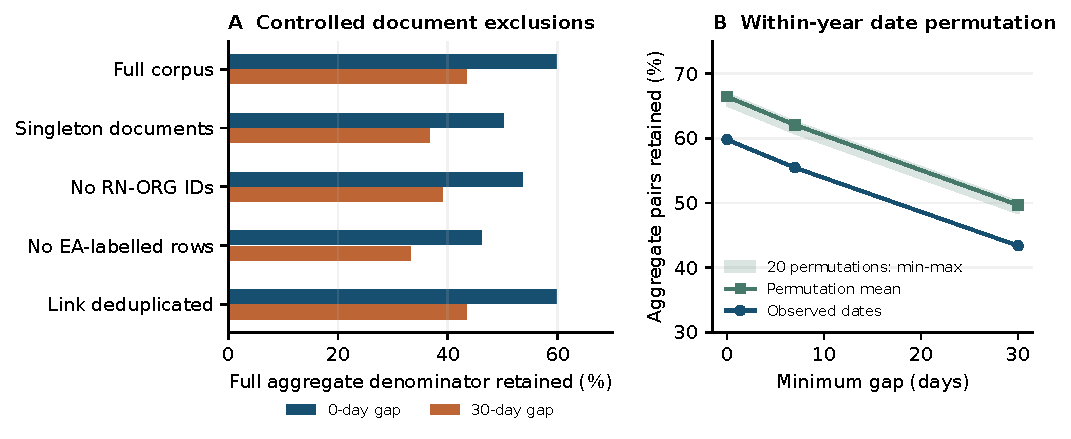
\includegraphics[width=\linewidth]{figures/sensitivity.pdf}
\caption{Document exclusions use the full aggregate denominator (A). Within-year date permutations preserve the document-date multiset; the shaded band shows the minimum and maximum across twenty specified seeds (B).}\label{fig:sensitivity}\end{figure}

The source-linked threshold makes the calculation inspectable. The illustration rule selects the first identifier-ordered pair in each year admitting a seven-day route, lacking a direct contact, and failing at thirty days. In 1771 it selects John Foxcroft to Samuel Rhoads Sr., through Benjamin Franklin. The two recorded documents are dated January 14 and February 10, a 27-day separation. The full-year model has no admissible route for that pair at 28 days. Figure~\ref{fig:witness} exposes both records. This establishes a model-specific temporal threshold; it supplies no evidence that Franklin passed Foxcroft's information to Rhoads.

\begin{figure}[htbp]\centering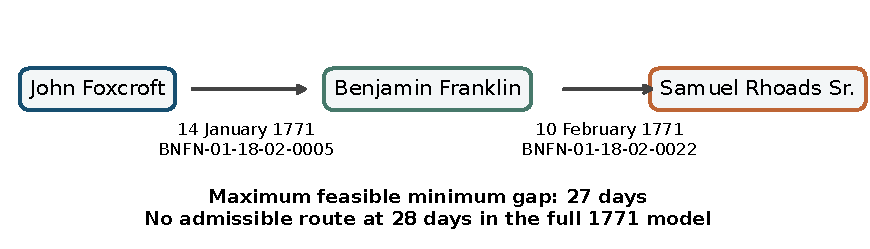
\includegraphics[width=\linewidth]{figures/witness.pdf}
\caption{An illustrative metadata route selected by the stated rule. Document identifiers and dates support a 27-day critical gap in the model. The arrows do not assert content transmission or observed receipt.}\label{fig:witness}\end{figure}

\FloatBarrier
\section{Interpretation, reuse, and limits}
The audit changes the evidential role of a network figure. A historian can distinguish a relationship documented somewhere in the year, a chronology compatible with successive documents, and a chronology compatible with a stated handoff restriction. Each is a legitimate analytical object. A synthetic narrative gains precision when its claim is attached to the corresponding object and its supporting records.

The most useful output can be a research question directed back to an edition: when was the incoming document received, and what connects it to the outgoing communication? A critical gap identifies how much temporal room the recorded routes possess. It can prioritize inspection of endorsements, receipt notations, replies, or references to enclosures. Establishing actual transmission requires those records and their contents; increasing computational precision alone cannot supply them.

Practical reuse includes archive interfaces, classroom network demonstrations, and source-grounded research software. A query can return its documentary route, window, projection rule, and gap setting alongside a visualization. A commercial implementation could package such evidence inspection for publishers or research platforms. This study evaluates computational feasibility and documentary transparency; it contains no customer-validation study or claim of patentable algorithmic invention.

Several limits govern the results. Associated dates may be editorially supplied and need not be dispatch dates. The CSV provides neither receipt times nor sufficient information to estimate route-specific transport durations. Uniform gaps summarize sensitivity rather than geography. Identifier reconciliation and corporate identities affect the graph; the reported exclusions expose some consequences without resolving those interpretive choices. Annual windows omit cross-year routes. Unrecorded correspondence, oral exchange, newspapers, and shared meetings can connect people outside this documentary graph.

\begin{samepage}
The empirical finding is bounded but conclusive: for the frozen compilation and declared route model, aggregation and handoff assumptions produce materially different reachability sets. DispatchGap returns documents through which their significance can be investigated and makes the passage from a dated tie to a proposed communication route explicit and criticizable.

\paragraph{Availability.} Code, pinned metadata, result tables, tests, and figure-generation scripts are released at \url{https://github.com/shi1720/dispatchgap}. Software is MIT licensed; the Rotunda dataset retains its CC BY 4.0 attribution and license. Analysis uses the Python standard library; plotting dependencies are separately specified.
\paragraph{Disclosure.} Generative AI assisted literature discovery, software development, analysis, visualization, and drafting.
\end{samepage}

\begin{thebibliography}{9}\small
\bibitem{rotunda} Rotunda, University of Virginia Press. 2026. \emph{Revolutionary Networks: Correspondence Metadata, 1771--1783}. Dataset, commit dacbbff257a769740c5bf8e25c6fb0a5212bf671. \url{https://github.com/rotunda-uvap/revolutionary-networks}.
\bibitem{holme} Holme, Petter, and Jari Saram\"aki. 2012. ``Temporal Networks.'' \emph{Physics Reports} 519(3): 97--125. \url{https://doi.org/10.1016/j.physrep.2012.03.001}.
\bibitem{bazgan} Bazgan, Cristina, Johannes Kager, Clemens Thielen, and Daniel Vanderpooten. 2025. ``A General Label Setting Algorithm and Tractability Analysis for the Multiobjective Temporal Shortest Path Problem.'' \emph{Networks} 85(1): 76--90. \url{https://doi.org/10.1002/net.22253}.
\bibitem{ahnert} Ahnert, Ruth, Sebastian E. Ahnert, Catherine Nicole Coleman, and Scott B. Weingart. 2020. \emph{The Network Turn: Changing Perspectives in the Humanities}. Cambridge University Press. \url{https://doi.org/10.1017/9781108866804}.
\bibitem{leskinen} Leskinen, Petri, Javier Ure\~na-Carrion, Jouni Tuominen, Mikko Kivel\"a, and Eero Hyv\"onen. 2026. ``Knowledge Graphs and Data Services for Studying Historical Epistolary Data in Network Science on the Semantic Web.'' \emph{Semantic Web}. Published online June 6. \url{https://doi.org/10.1177/22104968261452976}.
\bibitem{urena} Ure\~na-Carrion, Javier, Petri Leskinen, Jouni Tuominen, Charles van den Heuvel, Eero Hyv\"onen, and Mikko Kivel\"a. 2022. ``Communication Now and Then: Analyzing the Republic of Letters as a Communication Network.'' \emph{Applied Network Science} 7: 26. \url{https://doi.org/10.1007/s41109-022-00463-1}.
\bibitem{alassi} Alassi, Sepideh, and Lukas Rosenthaler. 2024. ``Semantic Precision: Crafting RDF-Based Digital Editions for Unveiling the Layers of Historical Correspondence.'' \emph{Digital Scholarship in the Humanities} 39(3): 813--835. \url{https://doi.org/10.1093/llc/fqae027}.
\bibitem{an} An, Yu Lee. 2026. ``Reconstructing Historical Events with CIDOC CRM.'' \emph{Anthology of Computers and the Humanities} 5. \url{https://doi.org/10.63744/AfxZkbfK4dXG}.
\bibitem{kane} Kane, Maeve. 2024. ```By Conversation with a Lady': Women's Correspondence Networks in the Founders Online Database.'' In \emph{American Revolutions in the Digital Age}, edited by Nora Slonimsky, Mark Boonshoft, and Ben Wright, 184--200. Cornell University Press. \url{https://www.jstor.org/stable/10.7591/jj.24541210.14}.
\end{thebibliography}

\clearpage\appendix
\section*{Appendix: complete annual results}
\begin{table}[htbp]\centering\small
\caption{Annual counts. Documents have nonempty endpoint identifier sets. Contacts exclude self-contacts and preserve originating document identifiers.}\label{tab:annual}
\begin{tabular}{rrrrrrr}\toprule Year&Documents&Nodes&Contacts&Aggregate&Gap 0&Gap 30\\\midrule
1771&270&168&274&3,097&1,697&1,449\\
1772&377&199&388&6,544&3,847&3,305\\
1773&480&220&494&6,834&3,876&3,402\\
1774&498&260&543&8,444&3,806&3,196\\
1775&1,400&499&1,491&78,897&35,120&22,031\\
1776&2,606&568&2,949&128,547&77,564&58,883\\
1777&4,387&850&5,507&311,099&178,882&136,394\\
1778&5,308&1,183&6,802&553,967&327,843&238,051\\
1779&5,195&1,022&5,510&464,518&292,761&214,846\\
1780&5,596&1,090&5,727&529,097&317,299&227,703\\
1781&5,843&1,189&6,031&603,493&363,533&254,446\\
1782&4,820&1,016&5,030&446,317&274,758&199,051\\
1783&3,879&1,051&4,171&438,107&258,668&189,913\\
\bottomrule\end{tabular}
\end{table}
\begin{table}[htbp]\centering\small
\caption{Pooled exclusion results. The denominator remains the full corpus's 3,578,961 aggregate source-year pairs. Exclusions are sensitivity specifications, not ratings of documentary quality.}
\begin{tabular}{lrrr}\toprule Profile&Gap 0&Gap 7&Gap 30\\\midrule
Singleton documents&1,797,807&1,662,318&1,309,849\\
No RN-ORG identifiers&1,920,351&1,780,719&1,399,404\\
No EA-labelled rows&1,652,330&1,530,484&1,187,346\\
Source-link deduplicated&2,139,218&1,984,062&1,552,300\\
\bottomrule\end{tabular}
\end{table}
\end{document}
